\documentclass[t]{beamer}

% xcolor and define colors -------------------------
\usepackage{xcolor}

% https://www.viget.com/articles/color-contrast/
\definecolor{purple}{HTML}{5601A4}
\definecolor{navy}{HTML}{0D3D56}
\definecolor{ruby}{HTML}{9a2515}
\definecolor{alice}{HTML}{107895}
\definecolor{daisy}{HTML}{EBC944}
\definecolor{coral}{HTML}{F26D21}
\definecolor{kelly}{HTML}{829356}
\definecolor{cranberry}{HTML}{E64173}
\definecolor{jet}{HTML}{131516}
\definecolor{asher}{HTML}{555F61}
\definecolor{slate}{HTML}{314F4F}

% Mixtape Sessions
\definecolor{picton-blue}{HTML}{00b7ff}
\definecolor{violet-red}{HTML}{ff3881}
\definecolor{sun}{HTML}{ffaf18}
\definecolor{electric-violet}{HTML}{871EFF}

\newcommand\pictonBlue[1]{{\color{picton-blue}#1}}
\newcommand\sun[1]{{\color{sun}#1}}
\newcommand\electricViolet[1]{{\color{electric-violet}#1}}
\newcommand\violetRed[1]{{\color{violet-red}#1}}

\newcommand\bgPictonBlue[1]{{\colorbox{picton-blue!20!white}{#1}}}
\newcommand\bgSun[1]{{\colorbox{sun!20!white}{#1}}}
\newcommand\bgElectricViolet[1]{{\colorbox{electric-violet!20!white}{#1}}}
\newcommand\bgVioletRed[1]{{\colorbox{violet-red!20!white}{#1}}}

\def\code#1{\texttt{#1}}

% Main theme colors
\definecolor{accent}{HTML}{00b7ff}
\definecolor{accent2}{HTML}{871EFF}
\definecolor{gray100}{HTML}{f3f4f6}
\definecolor{gray800}{HTML}{1F292D}


% Beamer Options -------------------------------------

% Background
\setbeamercolor{background canvas}{bg = white}

% Change text margins
\setbeamersize{text margin left = 15pt, text margin right = 15pt} 

% \alert
\setbeamercolor{alerted text}{fg = accent2}

% Frame title
\setbeamercolor{frametitle}{bg = white, fg = jet}
\setbeamercolor{framesubtitle}{bg = white, fg = accent}
\setbeamerfont{framesubtitle}{size = \small, shape = \itshape}

% Block
\setbeamercolor{block title}{fg = white, bg = accent2}
\setbeamercolor{block body}{fg = gray800, bg = gray100}

% Title page
\setbeamercolor{title}{fg = gray800}
\setbeamercolor{subtitle}{fg = accent}

%% Custom \maketitle and \titlepage
\setbeamertemplate{title page}
{
    %\begin{centering}
        \vspace{20mm}
        {\Large \usebeamerfont{title}\usebeamercolor[fg]{title}\inserttitle}\\
        {\large \itshape \usebeamerfont{subtitle}\usebeamercolor[fg]{subtitle}\insertsubtitle}\\ \vspace{10mm}
        {\insertauthor}\\
        {\color{asher}\small{\insertdate}}\\
    %\end{centering}
}

% Table of Contents
\setbeamercolor{section in toc}{fg = accent!70!jet}
\setbeamercolor{subsection in toc}{fg = jet}

% Button 
\setbeamercolor{button}{bg = accent}

% Remove navigation symbols
\setbeamertemplate{navigation symbols}{}

% Table and Figure captions
\setbeamercolor{caption}{fg=jet!70!white}
\setbeamercolor{caption name}{fg=jet}
\setbeamerfont{caption name}{shape = \itshape}

% Bullet points

%% Fix spacing between items
\let\olditemize=\itemize 
\let\endolditemize=\enditemize 
\renewenvironment{itemize}{\vspace{0.25em}\olditemize \itemsep0.25em}{\endolditemize}

%% Fix left-margins
\settowidth{\leftmargini}{\usebeamertemplate{itemize item}}
\addtolength{\leftmargini}{\labelsep}

%% enumerate item color
\setbeamercolor{enumerate item}{fg = accent}
\setbeamerfont{enumerate item}{size = \small}
\setbeamertemplate{enumerate item}{\insertenumlabel.}

%% itemize
\setbeamercolor{itemize item}{fg = accent!70!white}
\setbeamerfont{itemize item}{size = \small}
\setbeamertemplate{itemize item}[circle]

%% right arrow for subitems
\setbeamercolor{itemize subitem}{fg = accent!60!white}
\setbeamerfont{itemize subitem}{size = \small}
\setbeamertemplate{itemize subitem}{$\rightarrow$}

\setbeamertemplate{itemize subsubitem}[square]
\setbeamercolor{itemize subsubitem}{fg = jet}
\setbeamerfont{itemize subsubitem}{size = \small}








% Links ----------------------------------------------

\usepackage{hyperref}
\hypersetup{
  colorlinks = true,
  linkcolor = accent2,
  filecolor = accent2,
  urlcolor = accent2,
  citecolor = accent2,
}


% Line spacing --------------------------------------
\usepackage{setspace}
\setstretch{1.35}


% \begin{columns} -----------------------------------
\usepackage{multicol}


% Fonts ---------------------------------------------
% Beamer Option to use custom fonts
\usefonttheme{professionalfonts}

% \usepackage[utopia, smallerops, varg]{newtxmath}
% \usepackage{utopia}
\usepackage[sfdefault,light]{roboto}

% Small adjustments to text kerning
\usepackage{microtype}



% Remove annoying over-full box warnings -----------
\vfuzz2pt 
\hfuzz2pt


% Table of Contents with Sections
\setbeamerfont{myTOC}{series=\bfseries, size=\Large}
\AtBeginSection[]{
        \frame{
            \frametitle{Roadmap}
            \tableofcontents[current]   
        }
    }


% Tables -------------------------------------------
% Tables too big
% \begin{adjustbox}{width = 1.2\textwidth, center}
\usepackage{adjustbox}
\usepackage{array}
\usepackage{threeparttable, booktabs, adjustbox}
    
% Fix \input with tables
% \input fails when \\ is at end of external .tex file
\makeatletter
\let\input\@@input
\makeatother

% Tables too narrow
% \begin{tabularx}{\linewidth}{cols}
% col-types: X - center, L - left, R -right
% Relative scale: >{\hsize=.8\hsize}X/L/R
\usepackage{tabularx}
\newcolumntype{L}{>{\raggedright\arraybackslash}X}
\newcolumntype{R}{>{\raggedleft\arraybackslash}X}
\newcolumntype{C}{>{\centering\arraybackslash}X}

% Figures

% \imageframe{img_name} -----------------------------
% from https://github.com/mattjetwell/cousteau
\newcommand{\imageframe}[1]{%
    \begin{frame}[plain]
        \begin{tikzpicture}[remember picture, overlay]
            \node[at = (current page.center), xshift = 0cm] (cover) {%
                \includegraphics[keepaspectratio, width=\paperwidth, height=\paperheight]{#1}
            };
        \end{tikzpicture}
    \end{frame}%
}

% subfigures
\usepackage{subfigure}


% Highlight slide -----------------------------------
% \begin{transitionframe} Text \end{transitionframe}
% from paulgp's beamer tips
\newenvironment{transitionframe}{
    \setbeamercolor{background canvas}{bg=accent!40!black}
    \begin{frame}\color{accent!10!white}\LARGE\centering
}{
    \end{frame}
}


% Table Highlighting --------------------------------
% Create top-left and bottom-right markets in tabular cells with a unique matching id and these commands will outline those cells
\usepackage[beamer,customcolors]{hf-tikz}
\usetikzlibrary{calc}
\usetikzlibrary{fit,shapes.misc}

% To set the hypothesis highlighting boxes red.
\newcommand\marktopleft[1]{%
    \tikz[overlay,remember picture] 
        \node (marker-#1-a) at (0,1.5ex) {};%
}
\newcommand\markbottomright[1]{%
    \tikz[overlay,remember picture] 
        \node (marker-#1-b) at (0,0) {};%
    \tikz[accent!80!jet, ultra thick, overlay, remember picture, inner sep=4pt]
        \node[draw, rectangle, fit=(marker-#1-a.center) (marker-#1-b.center)] {};%
}


% DAGS ----------------------------------------------
\usepackage{tikz}
\usetikzlibrary{shapes,decorations,arrows,calc,arrows.meta,fit,positioning}
% Tikz settings optimized for causal graphs.
\tikzset{
    -Latex,auto,node distance =1 cm and 1 cm,semithick,
    state/.style ={ellipse, draw, minimum width = 0.7 cm},
    point/.style = {circle, draw, inner sep=0.04cm,fill,node contents={}},
    bidirected/.style={Latex-Latex,dashed},
    el/.style = {inner sep=2pt, align=left, sloped}
}


% Beamer tricks -------------------------------------
% Make \pause work in align environments
\makeatletter
\renewrobustcmd{\beamer@@pause}[1][]{%
  \unless\ifmeasuring@%
  \ifblank{#1}%
    {\stepcounter{beamerpauses}}%
    {\setcounter{beamerpauses}{#1}}%
  \onslide<\value{beamerpauses}->\relax%
  \fi%
}
\makeatother


\begin{document}

% Adjust spacing with equations
\setlength{\abovedisplayskip}{5pt}
\setlength{\belowdisplayskip}{5pt}
\setlength{\abovedisplayshortskip}{5pt}
\setlength{\belowdisplayshortskip}{5pt}

\imageframe{./lecture_includes/cover.png}

\section{Introductions}

\subsection{Me and This Course}
\begin{frame}{Who Am I?}

The Groos Family Assistant Professor of Economics, Brown University\pause

A big fan of instrumental variable methods:\pause
\begin{itemize}
  \item Lottery- and non-lottery IVs in studies of educational quality \\ {\scriptsize \textcolor{red!75!green!50!blue!25!gray}{(Angrist et al. 2016, 2017, 2021, 2022; Abdulkadiro\u{g}lu et al. 2016)}}
  \item Quasi-experimental evaluations of healthcare quality \\ {\scriptsize \textcolor{red!75!green!50!blue!25!gray}{(Hull 2020; Abaluck et al. 2021, 2022)}}
  \item IV-based analyses of discrimination and bias \\ {\scriptsize \textcolor{red!75!green!50!blue!25!gray}{(Arnold et al. 2020, 2021, 2022; Hull 2021; Bohren et al. 2022)}}

  \item \bgVioletRed{Shift-share instruments (SSIV) and related designs} \\ {\scriptsize \textcolor{red!75!green!50!blue!25!gray}{(Borusyak et al. 2022; Borusyak and Hull 2021, 2022; Goldsmith-Pinkham et al. 2022)}}
\end{itemize}

\end{frame}

\begin{frame}{What is This Course?}

A one-day intensive on SSIV, focusing on recent practical advances

\begin{itemize}
  \item Highlighting key points on identification, estimation, and inference
  \item Emphasis on \emph{practical}: IV is meant to be used, not just studied!
\end{itemize}\pause\medskip

Two 90-minute lectures

\begin{itemize}
  \item Please ask questions in the Discord chat!
\end{itemize}\pause\medskip

One 45-minute coding lab
\begin{itemize}
  \item 25 min: you seeing how far you can get on your own, or with your classmate's help (use Discord rooms!)
  \item 20 min: me live-coding solutions in Stata (we will also post R code)
\end{itemize}

\end{frame}

\begin{frame}{Schedule}
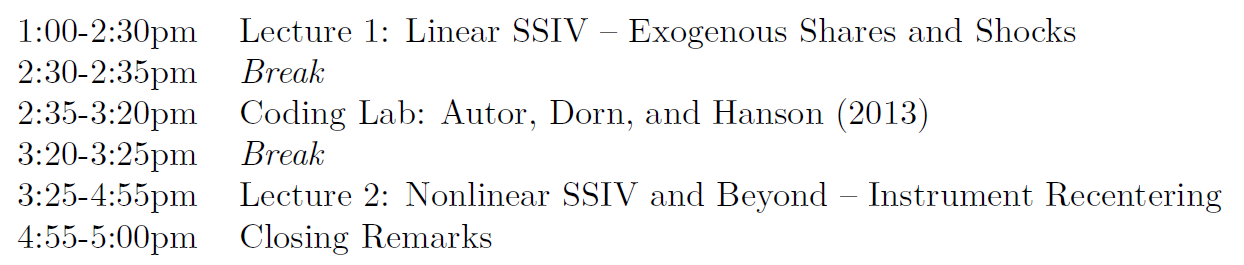
\includegraphics[scale=0.52]{./lecture_includes/schedule.png}
\end{frame}

\subsection{(Linear) SSIV}
\begin{frame}{What is a (Linear) SSIV?}

A weighted sum of a common set of \bgSun{shocks}, with weights reflecting heterogeneous \bgElectricViolet{exposure shares}:\hspace{0.25cm} $z_\ell=\sum_{n} \electricViolet{s_{\ell n}} \sun{g_n}$
\pause

\begin{itemize}
\item The shocks vary at a different ``level''  \bgSun{$n=1,\dots,N$} than the shares \bgElectricViolet{$\ell=1,\dots,L$}, where we also observe an outcome $y_\ell$ \& treatment $x_\ell$
\end{itemize}\pause\medskip

We want to use $z_\ell$ to estimate parameter $\beta$ of the model $y_\ell=\beta x_\ell+\varepsilon_\ell$
\pause
\begin{itemize}\itemsep0em
\item Could be a ``structural'' equation or a potential outcomes model
\item Could be misspecified, with heterogeneous treatment effects $\beta_\ell$
\item Could be a ``reduced form'' analysis, with $x_\ell=z_\ell$
\item Could have other included controls $w_\ell$ 
\end{itemize}
\pause\medskip

Key question: under what assumptions does this SSIV strategy ``work''?
\end{frame}

\begin{frame}{SSIV Examples}

\vspace*{-10mm}
\begin{equation*}
  \text{Instrument }
  z_\ell = \sum_{n}
  \tikz[baseline]{
      \node[draw=electric-violet,rounded corners,anchor=base] (m1)
      {$\electricViolet{s_{\ell n}}$};
      \node[above = 1mm of m1] (l1) {\small\color{electric-violet} shares};
      \draw[-,electric-violet] (l1) -- (m1);
  }
  \tikz[baseline]{
      \node[draw=sun,rounded corners,anchor=base] (m2)
      {$\sun{g_n}$};
      \node[above = 1mm of m2] (l2) {\small\color{sun} shocks};
      \draw[-,sun] (l2) -- (m2);
  }
  \text{ for model }
  y_\ell = \beta x_\ell + \gamma' w_\ell + \varepsilon_\ell
\end{equation*}
  
Bartik (1991); Blanchard and Katz (1992): 
	\begin{itemize}
	\item $\beta$ = inverse local labor supply elasticity 
	\item $x_\ell$ and $y_\ell$ = employment and wage growth in region $\ell$ 
	\item Need a labor demand shifter as an IV\pause\smallskip
	\item $\sun{g_n}$ = national growth of industry $n$
	\item $\electricViolet{s_{\ell n}}$ = lagged employment shares (of industry in a region)
	\item $z_\ell$ = predicted employment growth due to national industry trends
	\end{itemize}
\end{frame}

\begin{frame}{SSIV Examples}

\vspace*{-10mm}
\begin{equation*}
  \text{Instrument }
  z_\ell = \sum_{n}
  \tikz[baseline]{
      \node[draw=electric-violet,rounded corners,anchor=base] (m1)
      {$\electricViolet{s_{\ell n}}$};
      \node[above = 1mm of m1] (l1) {\small\color{electric-violet} shares};
      \draw[-,electric-violet] (l1) -- (m1);
  }
  \tikz[baseline]{
      \node[draw=sun,rounded corners,anchor=base] (m2)
      {$\sun{g_n}$};
      \node[above = 1mm of m2] (l2) {\small\color{sun} shocks};
      \draw[-,sun] (l2) -- (m2);
  }
  \text{ for model }
  y_\ell = \beta x_\ell + \gamma' w_\ell + \varepsilon_\ell
\end{equation*}

Autor, Dorn, and Hanson (2013, ADH):
	\begin{itemize}
	\item $x_\ell$ = growth of import competition in region $\ell$
	\item $y_\ell$ = growth of manuf. employment, unemployment, etc.\smallskip
	\item $\sun{g_n}$ = growth of China exports in manufacturing industry $n$ to 8 other (i.e. non-U.S.) countries
	\item $\electricViolet{s_{\ell n}}$ = 10-year lagged employment shares (over total employment)
	\item $z_\ell$ = predicted growth of import competition
	\end{itemize}
\end{frame}

\begin{frame}{SSIV Examples}
\vspace*{-10mm}
\begin{equation*}
  \text{Instrument }
  z_\ell = \sum_{n}
  \tikz[baseline]{
      \node[draw=electric-violet,rounded corners,anchor=base] (m1)
      {$\electricViolet{s_{\ell n}}$};
      \node[above = 1mm of m1] (l1) {\small\color{electric-violet} shares};
      \draw[-,electric-violet] (l1) -- (m1);
  }
  \tikz[baseline]{
      \node[draw=sun,rounded corners,anchor=base] (m2)
      {$\sun{g_n}$};
      \node[above = 1mm of m2] (l2) {\small\color{sun} shocks};
      \draw[-,sun] (l2) -- (m2);
  }
  \text{ for model }
  y_\ell = \beta x_\ell + \gamma' w_\ell + \varepsilon_\ell
\end{equation*}

``Enclave instrument'', e.g. Card (2009) 
	\begin{itemize}
	\item $\beta$ = inverse elasticity of substitution between native and immigrant labor of some skill level (need a relative labor supply instrument)
	\item $x_\ell$ and $y_\ell$ = relative employment and wage in region $\ell$\smallskip
	\item $\sun{g_n}$ = national immigration growth from origin country $n$
	\item $\electricViolet{s_{\ell n}}$ = lagged shares of migrants from origin $n$ in region $\ell$
	\item $z_\ell$ = share of migrants predicted from enclaves \& recent growth
	\end{itemize}
\end{frame}

\begin{frame}{SSIV Examples}
\vspace*{-10mm}
\begin{equation*}
  \text{Instrument }
  z_\ell = \sum_{n}
  \tikz[baseline]{
      \node[draw=electric-violet,rounded corners,anchor=base] (m1)
      {$\electricViolet{s_{\ell n}}$};
      \node[above = 1mm of m1] (l1) {\small\color{electric-violet} shares};
      \draw[-,electric-violet] (l1) -- (m1);
  }
  \tikz[baseline]{
      \node[draw=sun,rounded corners,anchor=base] (m2)
      {$\sun{g_n}$};
      \node[above = 1mm of m2] (l2) {\small\color{sun} shocks};
      \draw[-,sun] (l2) -- (m2);
  }
  \text{ for model }
  y_\ell = \beta x_\ell + \gamma' w_\ell + \varepsilon_\ell
\end{equation*}

Hummels et al. (2014) on offshoring: 
	\begin{itemize}
	\item $x_\ell$ = imports by Danish firm $\ell$, $y_\ell$ = wages
	\item $\sun{g_n}$ = changes in transport costs by $n = \text{(product, country)}$
	\item $\electricViolet{s_{\ell n}}$ = lagged import shares
	\end{itemize}
\end{frame}

\begin{frame}{What Do We Do With This?}

Of course we can always run IV with such $z_\ell$ ... but what does the corresponding estimand \emph{identify}?
\bigskip\pause

Recall IV validity condition: $E\left[\frac{1}{L}\sum_\ell z_\ell \varepsilon_\ell\right]=0$ for model residual $\varepsilon_\ell$\smallskip
\begin{itemize}
\item Looks a little different than normal because we're not assuming \emph{i.i.d.} sampling, i.e. $E\left[\frac{1}{L}\sum_\ell z_\ell \varepsilon_\ell\right]=E[z_\ell\varepsilon_\ell]$  (you'll see why soon!)
\end{itemize}
\bigskip\pause

What properties of shocks and shares make this condition hold?
\smallskip
\begin{itemize}
\item Is SSIV like a natural experiment? A diff-in-diff? Something new?
\item Since $z_\ell$ combines multiple sources of variation, it can be difficult to think about it being randomly assigned across $\ell$...
\end{itemize}
\end{frame}

\section{Shock Exogeneity}

\subsection{Motivation}

\begin{frame}{Exogenous Shocks in Industry-Level Regressions}
Acemoglu-Autor-Dorn-Hanson-Price (AADHP, 2016) look at the effects of import competition with China on US manufacturing  \emph{industries}:
$$\Delta\log Emp_{nt}=\alpha+\beta \Delta IP_{nt}+\varepsilon_{nt}, $$
where $\Delta IP_{nt}$ measures growth in import penetration from China in industry $n$, and $\varepsilon_{nt}$ captures industry demand/productivity shocks
\pause\bigskip

Two Key Problems with OLS estimation:\smallskip
\begin{enumerate}
\item Endogeneity of $\Delta IP_{nt}$: OLS is not consistent for $\beta$
\smallskip
\item GE spillovers: $\beta$ does not capture aggregate effects
\end{enumerate}
\end{frame}


\begin{frame}[t]{Problem 1: Endogeneity of $\Delta IP_{nt}$}
\vspace{-0.5cm}
$$\Delta\log Emp_{nt}=\alpha+\beta \Delta IP_{nt}+\varepsilon_{nt}$$

$\Delta IP_{nt}$ is driven by productivity shocks in China, but also potentially by productivity and demand shocks in the US %(+, --, +)
\smallskip
\begin{itemize}
\item $\varepsilon_{nt}$ captures productivity and demand shocks in the US %(+, +)
\end{itemize}

\pause
AADHP instrument $\Delta IP_{nt}$ with $\Delta IPO_{nt}$, measuring average Chinese import penetration growth in 8 non-US countries\smallskip\pause
	\begin{itemize}
	\item Relevance: both  $\Delta IP_{nt}$ and $\Delta IPO_{nt}$ are driven by the same Chinese productivity shocks
	\item Validity: local productivity/demand shocks in the US are uncorrelated with those of other countries (entering $\Delta IPO_{nt}$)
	\end{itemize}
\end{frame}

\begin{frame}{Identification from a Natural Experiment}
\vspace{-0.2cm}
Suppose $\Delta IPO_{nt}$ is as-good-as-randomly assigned, as in a RCT: 
\begin{align*}
E[\Delta IPO_{nt}\mid \mathcal{I]}=\mu\qquad\text{for all }n,t
\end{align*}

where $\mathcal{I}=\left\{\varepsilon_{nt},\text{pre-trends, balance variables},\dots\right\}$
\pause\bigskip


Consistent IV estimation then follows from many observations of $nt$, with sufficiently independent variation in $\Delta IPO_{nt}$
\end{frame}

\begin{frame}{Identification from a Natural Experiment}
Can relax to add observables capturing systematic variation:
\begin{align*}
E[\Delta IPO_{nt}\mid \mathcal{I}]=q_{nt}^\prime\mu\qquad\text{for all }n,t
\end{align*}

where $q_{nt}$ may include:
\smallskip
\begin{itemize}
\item period FE, isolating within-period variation in the shocks \smallskip
\item FE of 10 broad sectors, isolating within-sector variation, etc. 
\end{itemize}\smallskip\pause
We would then just want to control for $q_{nt}$ in the industry-level IV
\end{frame}

\begin{frame}{Problem 2: GE Spillovers}
\vspace{-0.2cm}
Spillovers across different industries are likely important:
	\begin{itemize}
	\item When employment  shrinks in industry $n$ after a negative shock, aggregate employment may or may not respond
	\pause\smallskip
	\item In a flexible labor market, comparing wages of similar workers across industries does not make sense
	%\pause\smallskip
	%\item NILF: not well-defined at the industry level % KB maybe take out of here, somewhat distinct
	\pause\medskip
	\end{itemize}

\end{frame}

\begin{frame}{Problem 2: GE Spillovers}

ADH Solution: specify the outcome equation for local labor markets %instead of industries% KB here can connect to two-tier randomization in devt?
\begin{itemize}
%	\item To have many observations, compare \emph{local} labor market markets
%	\pause\smallskip
\item Works if local economies are isolated ``islands'' \\(simple model in Adao-Kolesar-Morales 2019; richer structure of spatial spillovers in Adao-Arkolakis-Esposito 2020)
\pause\medskip
\end{itemize}

But correct specification is not the same as identification!
	\begin{itemize}
	\item Key point: the same industry-level natural experiment can be used to estimate a regional specification, via SSIV
%	\smallskip
%	\item Also need individual labor markets to be concentrated in a small number of industries, to have enough variation in SSIV
	\end{itemize}
\end{frame}

\subsection{Borusyak et al. (2022)}
\begin{frame}{Borusyak, Hull, and Jaravel (BHJ; 2022)}

Consider the SSIV estimator of $y_\ell=\beta x_\ell+\gamma'w_\ell+\varepsilon_\ell$ instrumented by $z_\ell=\sum_n s_{\ell n}g_n$ and, for now, $\sum_n s_{\ell n}=1$ for all $\ell$

\smallskip
	\begin{itemize}
	\item Reduced-form allowed: $x_\ell=z_\ell$ \smallskip
	\item Only the shift-share structure of $z_\ell$ matters; $x_\ell$ can be anything 
	\smallskip
	\item Note: view $g_n$ as stochastic, so can't assume $z_\ell$ is iid
	\end{itemize}

\medskip\pause
E.g. $g_n= \Delta IPO_{n}$ aggregated w/mfg employment shares $s_{\ell n}$\smallskip
\begin{itemize}
\item Can we leverage a natural experiment in $g_n$, as before?
\end{itemize}
\medskip\pause
\end{frame}

\begin{frame}{Leveraging $g_n$}{Shift-Share Estimand}
\vspace{-0.2cm}
Consider the SSIV estimator of $y_\ell=\beta x_\ell+\gamma'w_\ell+\varepsilon_\ell$ instrumented by $z_\ell=\sum_n s_{\ell n}g_n$ and, for now, $\sum_n s_{\ell n}=1$ for all $\ell$

\vspace{5mm}
First step: note that by the FWL thm. the estimator can be written
\begin{align*}
\hat{\beta}=\frac{\sum_\ell z_\ell y_\ell^\perp}{\sum_\ell z_\ell x_\ell^\perp}=\frac{\sum_\ell \sum_n s_{\ell n}g_n y_\ell^\perp}{\sum_\ell \sum_n s_{\ell n}g_n x_\ell^\perp}
\end{align*}
where $v_\ell^\perp$ denotes sample residuals from regressing $v_\ell$ on $w_\ell$

\end{frame}


\begin{frame}{Leveraging $g_n$}{BHJ Numerical Equivalence}
\vspace{-0.2cm}
 BHJ show $\hat{\beta}$ can be obtained from a %just-identified 
shock-level IV procedure that uses $g_n$ to instrument for a shock-level ``aggregate'' of the treatment:\pause

\begin{align*}
\hat{\beta}=\frac{\frac{1}{L}\sum_\ell \sum_n s_{\ell n} g_n y_\ell^\perp}{\frac{1}{L}\sum_\ell \sum_n s_{\ell n} g_n x_\ell^\perp}=\pause\frac{\sum_n g_n \sum_\ell\frac{1}{L}  s_{\ell n} y_\ell^\perp}{\sum_n g_n\sum_\ell\frac{1}{L}  s_{\ell n}  x_\ell^\perp}=\pause\frac{\sum_n s_n g_n \bar{y}_n^\perp}{\sum_n s_n g_n \bar{x}_n^\perp},
\end{align*}

\vspace{2.5mm}
where $s_n=\frac{1}{L}\sum_\ell s_{\ell n}$ are weights capturing the average importance of shock $n$, and $\bar{v}_n=\frac{\sum_\ell s_{\ell n} v_\ell}{\sum_\ell s_{\ell n}}$ is an exposure-weighted average of $v_\ell$\medskip\pause
\end{frame}


\begin{frame}{Leveraging $g_n$}{BHJ Numerical Equivalence}
\vspace{-7.5mm}
$$
\hat{\beta}= \frac{\sum_n s_n g_n \bar{y}_n^\perp}{\sum_n s_n g_n \bar{x}_n^\perp}
$$

\vspace{2.5mm}
The IV estimate from the original shock-level IV procedure is equivalent to a ``industry-level'' IV regression with model $\bar{y}_n^\perp = \alpha + \bar{x}_n^\perp \beta + \bar{\epsilon}_n$ instrumented by $g_n$ with weights $s_n$.
\medskip

The residual $\bar\varepsilon_n$ of this shock-level IV procedure is the average residual of observations with a high share of $n$
\begin{itemize}
  \item E.g. in ADH, the average unobserved determinants of regional employment in regions most specialized in industry $n$
\end{itemize}

\pause
It follows that $\hat{\beta}$ is consistent iff this shock-level IV procedure is...

\end{frame}

\begin{frame}{BHJ Baseline Assumptions}

\vspace{-0.3cm}
 \textbf{A1} (Quasi-random shock assignment): $E[g_n\mid\bar{\varepsilon},s]=\mu$, for all $ n$

\begin{itemize}
  \item Each shock has the same expected value, conditional on the shock-level unobservables $\bar{\varepsilon}_n$ and average exposure $s_n$\pause

  \item Implies SSIV exogeneity, as $z_\ell=\mu+\sum_n s_{\ell n}(g_n-\mu)=\mu+\text{``noise''}$ 
\end{itemize}

\end{frame}

\begin{frame}{BHJ Baseline Assumptions}
\textbf{A2} (Many uncorrelated shocks):
\begin{itemize}
  \item  $E\left[\sum_n s_n^2\right]\rightarrow 0$: expected Herfindahl index of average shock exposure converges to zero (implies $N\rightarrow \infty$)

  \item $Cov(g_n,g_{n^\prime}\mid\bar{\varepsilon},s)=0$ for all $n^\prime\ne n$: shocks are mutually uncorrelated given the unobservables

  \pause
  \item Imply a shock-level law of large numbers: $\sum_n s_n g_n\bar{\varepsilon}_n\xrightarrow{p} 0$
\end{itemize}\medskip\pause
 
Both assumptions, while novel for SSIV, would be standard for a shock-level IV regression with weights $s_n$ and instrument $g_n$

\end{frame}

\begin{frame}{BHJ Extensions}
\vspace{-0.3cm}
\textbf{Conditional Quasi-Random Assignment}: $E[g_n\mid \bar{\varepsilon},q,s]=q_n^\prime \mu$ for some observed shock-level variables $q_n$\smallskip
\begin{itemize}
\item Consistency follows when $w_\ell = \sum_n s_{\ell n} q_n$ is controlled for in the IV
\end{itemize}\medskip\pause
\textbf{Weakly Mutually Correlated Shocks}: $g_n\mid (\bar{\varepsilon},q,s)$ are clustered or otherwise mutually dependent \smallskip
\begin{itemize}
\item Consistency follows when mutual correlation is not too strong
\end{itemize}\medskip\pause
 \textbf{Estimated Shocks}: $g_n=\sum_\ell w_{\ell n}g_{\ell n}$ proxies for an infeasible $g_n^*$\smallskip
\begin{itemize}
\item Consistency may require a ``leave-out'' adjustment: $z_\ell=\sum_\ell s_{\ell n}\tilde{g}_{\ell n}$ for $\tilde{g}_{\ell n}=\sum_{\ell^\prime\neq \ell} \omega_{\ell^\prime n}g_{\ell^\prime n}$ (akin to JIVE solution to many-IV bias) 
\end{itemize}

\end{frame}


\begin{frame}{BHJ Extensions (cont.)}
\vspace{-0.3cm}
\textbf{Panel Data}: Have $(y_{\ell t},x_{\ell t},s_{\ell n t},g_{n t})$ across $\ell=1,\dots,L$, $t=1,\dots,T$\smallskip
\begin{itemize}
\item Consistency can follow from either $N\rightarrow\infty$ or $T\rightarrow\infty$\smallskip
\item Unit fixed effects ``de-mean'' the shocks, if $s_{\ell n t}$ are time-invariant%\smallskip\pause
%\item Also see Jaeger et al. (2019) for dynamic biases in panel SSIVs
\end{itemize}\medskip\pause
\textbf{Heterogeneous Effects}: LATE theorem logic goes through
\begin{itemize}
\item Under a first-stage monotonicity condition, SSIV identifies a convex weighted average of heterogeneous treatment effects
\end{itemize}

\end{frame}

\begin{frame}{Practical Consideration 1: Incomplete Shares}{The Problem}

\vspace{-5mm}
So far we have assumed a constant sum-of-shares: $S_\ell\equiv\sum_n s_{\ell n}=1$\smallskip
\begin{itemize}
\item But in some settings, $S_\ell$ varies across $\ell$\smallskip
\item E.g. in ADH, $S_\ell$ is region $\ell$'s share of non-manufacturing emp.
\end{itemize}\bigskip\pause
 BHJ show that \textbf{A1}/\textbf{A2} are not enough for validity of $z_\ell$ in this case\smallskip
\begin{itemize}
\item Now $z_\ell=\sum_n s_{\ell n}\left(\mu+(g_n-\mu)\right)=\mu S_\ell+\sum_n s_{\ell n}(g_n-\mu)$\smallskip
\item So $z_\ell$ is mechanically correlated with $S_\ell$, which may be endogenous 
\end{itemize}


E.g. in ADH, Comparing locations with larger and smaller $z_\ell$ could be comparing places with larger manufacturing employment (Midwest vs. South)

\end{frame}

\begin{frame}{Practical Consideration 1: Incomplete Shares}{The Solution}

$$
z_\ell = \sum_n s_{\ell n}\left(\mu+(g_n-\mu)\right) = \mu S_\ell + \underbrace{\sum_n s_{\ell n}(g_n-\mu)}_{\text{Clean Shock Variation}}
$$

Controlling for the sum-of-shares $S_\ell$ isolates clean shock variation\smallskip

\begin{itemize}
\item Further controls are needed when \textbf{A1} only holds conditional on $q_n$; \\ e.g. in panels, $S_\ell$ should be interacted with time FE
\end{itemize}
\end{frame}

\begin{frame}{Practical Consideration 2: Exposure Clustering}{The Problem}
Ad\~{a}o, Kolesar, and Morales (2019) study a novel inference challenge when SSIV identification leverages quasi-random shocks \smallskip

\begin{itemize}
\item Observations with similar shares $s_{\ell 1,},\dots,s_{\ell N}$ are likely to have correlated $z_\ell$, even when observations are not ``clustered'' in conventional ways (e.g. by distance)\smallskip

\item When $\varepsilon_\ell$ is similarly clustered (e.g. when $\varepsilon_\ell=\sum_n s_{\ell n}\nu_n +\tilde{\varepsilon}_\ell$), large-sample distribution of $\hat{\beta}$ may not be well-approximated by standard central limit theorems (CLTs)
\end{itemize}
\end{frame}

\begin{frame}{Practical Consideration 2: Exposure Clustering}{The Solution}
Ad\~{a}o, Kolesar, and Morales then derive a new CLT + SEs to address ``exposure clustering''\medskip
\begin{itemize}
\item ``Design-based'': leverage \emph{iid}ness of shocks, not observations
\end{itemize}
\pause\bigskip
\end{frame}

\begin{frame}{Practical Consideration 2: Exposure Clustering}{The Solution}

BHJ use similar logic to show robust/clustered SEs can be valid when $\hat{\beta}$ is given by estimating the `industry-level' regression
\begin{align*}
\bar{y}_n^\perp = \alpha+\beta\bar{x}_n^\perp+q_n^\prime\tau+\bar{\varepsilon}_n^\perp,
\end{align*}
instrumenting $\bar{x}_n^\perp$ by $g_n$ and weighting by $s_n$
\smallskip\pause
\begin{itemize}
\item Numerically identical IV estimate, when controls include $\sum_n s_{\ell n} q_n$\smallskip
\item Clustering logic: valid SEs are obtained when estimating the IV at the level of identifying variation (here, shocks)
\end{itemize}\pause
Same logic applies to performing valid balance/pre-trend tests and evaluating first-stage strength of the instrument\smallskip
\end{frame}

\begin{frame}{SSIV with \emph{ssaggregate}}
Stata package \emph{ssaggregate} leverages the BHJ equivalence result: it translates data to the shock level, after which researchers can proceed with familiar estimation commands (install w/ \emph{ssc install ssaggregate})

\begin{center}
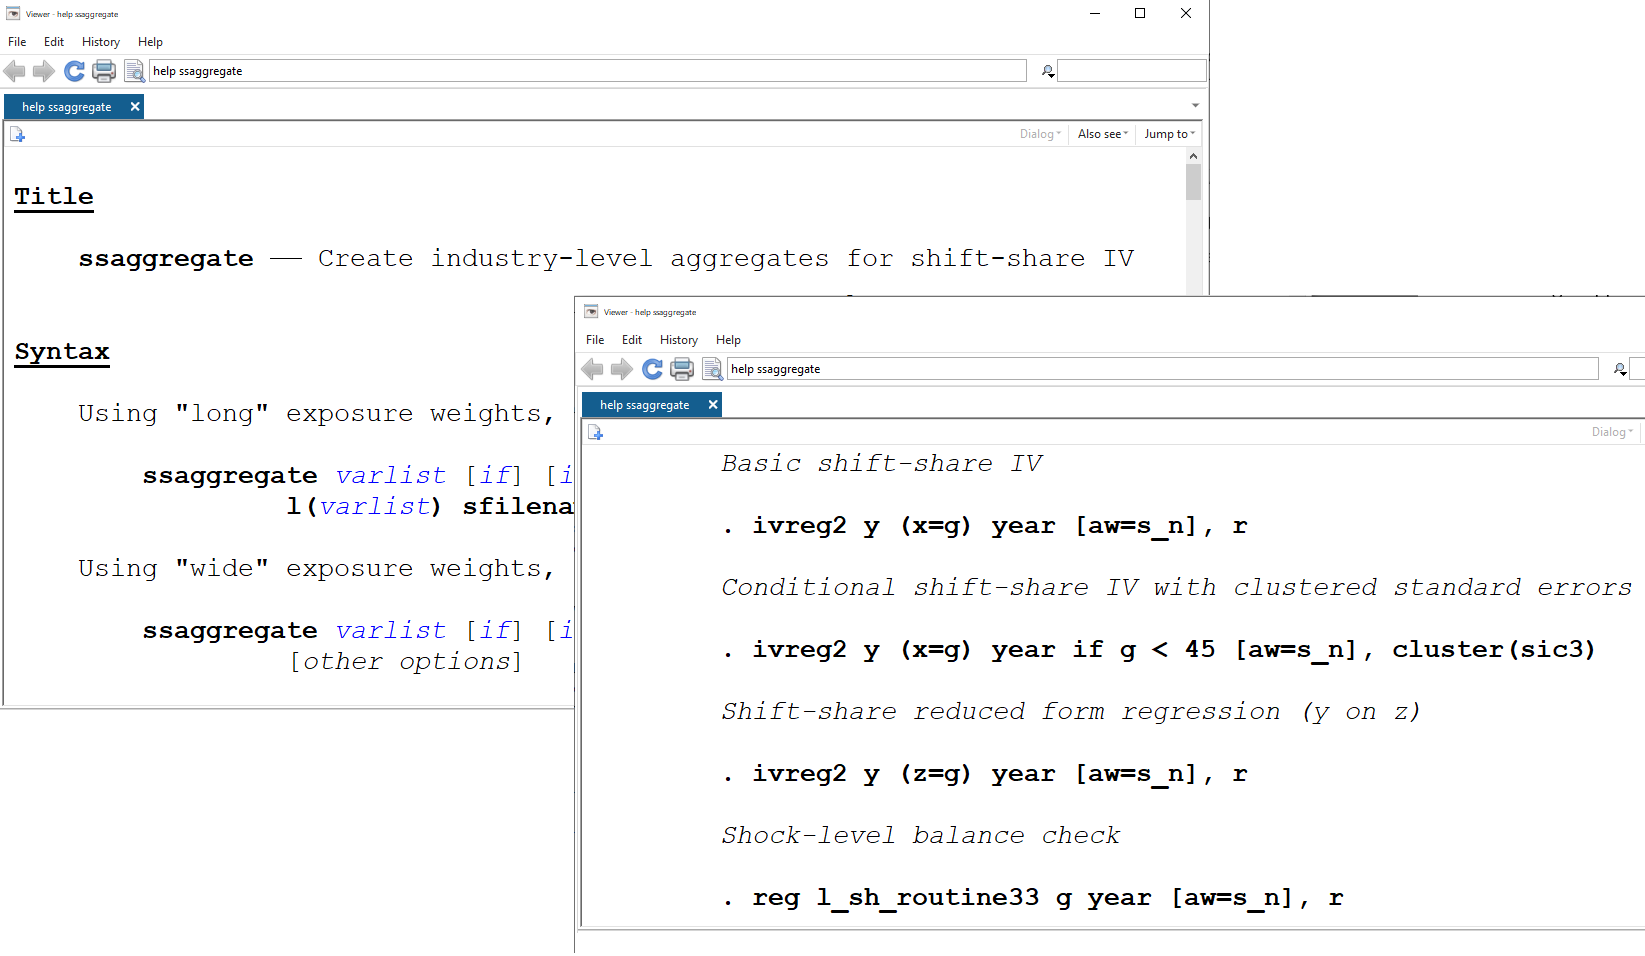
\includegraphics[height=0.6\textheight]{lecture_includes/ssaggregate.png}
\end{center}

\end{frame}


\begin{frame}{SSIV with \emph{ssaggregate}...in R!}
\vspace{-0.4cm}
Thanks to our own Kyle Butts, \emph{ssaggregate} is now available in R too!

\begin{center}

\includegraphics[height=0.7\textheight]{lecture_includes/ssaggregate_R.png}
\end{center}

Download at \url{https://github.com/kylebutts/ssaggregate}

\end{frame}

\begin{frame}{Application: ``The China Shock''} 
ADH study the effects of rising Chinese import competition on US commuting zones, 1991-2000 and 2000-2007
\smallskip
	\begin{itemize}
	\item Treatment $x_\ell$: local growth of Chinese imports  in \$1,000/worker (slightly different from AADHP and ADHS)\smallskip
	\item Main outcome $y_\ell$: local change in manufacturing emp. share
	\end{itemize}
	\pause\medskip
To address endogeneity challenge, use a SSIV $z_{\ell t}=\sum_n s_{\ell nt} g_{nt}$\smallskip
	\begin{itemize}
	\item $n$: 397 SIC4 manufacturing industries ($\times$ 2 periods)\smallskip
	\item $g_{nt}$: growth of Chinese imports in non-US economies per US worker \smallskip
	\item $s_{\ell nt}$: lagged share of mfg. industry $n$ in \emph{total} emp. of location $\ell$
	\end{itemize}
\end{frame}

\begin{frame}{ADH Revisited}
BHJ show how ADH can be seen as leveraging quasi-random shocks\smallskip
\begin{itemize}
	\item \emph{Ex ante} plausible: imagine random industry productivity shocks in China affecting imports in U.S. \& elsewhere
\end{itemize}

\end{frame}

\begin{frame}{ADH Revisited}{Plausability of \textbf{A1}/\textbf{A2}}

Evaluate \textbf{A1} by regional and industry-level balance tests\smallskip
\begin{itemize}
	\item Industry shocks are uncorrelated with observables
\end{itemize}

\smallskip\pause
Check sensitivity to adjusting for potential industry-level confounders:
\begin{itemize}
	\item Control for $w_{\ell t}=\sum_n s_{\ell nt} q_{nt}$, where $q_{nt}$ include period FE, sector FE, the Acemoglu et al. (2016) observables, ...
\end{itemize}
\medskip\pause

Evaluate \textbf{A2} by studying variation across industries\smallskip
	\begin{itemize}
	\item Effective sample size (1/HHI of $s_n$ weights): 58-192\smallskip
	\item Shocks appear mutually uncorrelated across SIC3 sectors
	\end{itemize}
\end{frame} 

\begin{frame}{BHJ do ADH: Shock-Level Balance}
\begin{center}
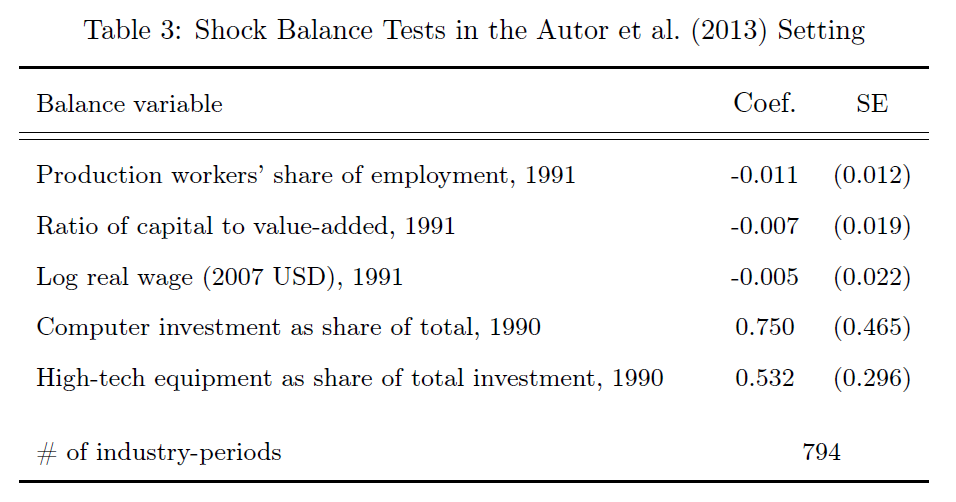
\includegraphics[scale=0.6]{lecture_includes/adh_balance.png}
\end{center}

No significant correlations between shocks and industry observables, controlling for year fixed effects
\end{frame}

\begin{frame}{BHJ do ADH: Manufacturing Employment}
\begin{center}
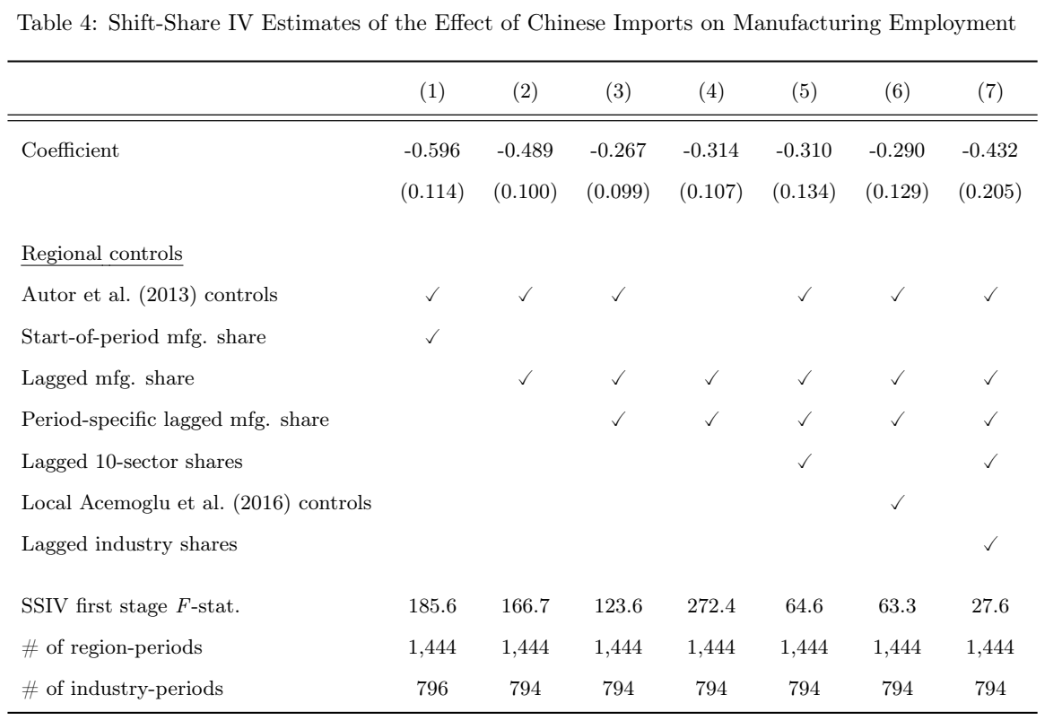
\includegraphics[scale=0.4]{lecture_includes/adh_bhj.png}
\end{center}
\end{frame}

\section{Share Exogeneity}

\subsection{Motivation}

\begin{frame}{The Mariel Boatlift as a Basic SSIV}
Card (1990) leverages a big migration ``push'' of low-skilled workers from Cuba to Miami, a Cuban-enclave. \pause 
Imagine instrumenting immigrant inflows by the lagged share of Cuban workers $s_{\ell, \text{Cuba}}$ in a diff-in-diff setup
\begin{itemize}
	\item Need parallel trends: regions with more/fewer Cuban workers on similar employment trends
\end{itemize}	

This can be viewed as a simple shift-share instrument: 
\vspace{-4mm}
$$s_{\ell, \text{Cuba}}\equiv s_{\ell,\text{Cuba}}\cdot 1+\sum_{n\ne\text{Cuba}} s_{\ell n}\cdot 0$$
\vspace{-6mm}\pause

If several migration origins had a push shock, we can pool them together with a more traditional SSIV...

\end{frame}

\subsection{Goldsmith-Pinkham et al. (2020)}

\begin{frame}{Goldsmith-Pinkham, Sorkin, and Swift (GPSS; 2020)} 

 GPSS view the set of $n$ and values of $g_n$ as fixed, so $z_\ell=\sum_n s_{\ell n} g_n$ is a linear combination of shares
\medskip\pause

They then also establish a numerical equivalence:
$\hat{\beta}$ can be obtained from an overidentified IV procedure that uses $N$ share instruments $s_{\ell n}$ and a weight matrix based on the shocks $g_n$



\end{frame}

\begin{frame}{Goldsmith-Pinkham, Sorkin, and Swift (GPSS; 2020)} 

Sufficient identifying assumption: shares $s_{\ell n}$ are exogenous for each $n$ (like parallel trends when $\varepsilon_\ell$ are unobserved trends)
\begin{align*}
E[\varepsilon_\ell\mid s_{\ell n}]=0,\text{ }\forall n \pause\implies E[\sum_\ell\nolimits z_\ell\varepsilon_\ell]=\sum_\ell\sum_n g_nE[s_{\ell n}]E[\varepsilon_\ell\mid s_{\ell n}]=0
\end{align*}

This is $N$ moment conditions at the level of observations, e.g. 38 for Card and 397 for ADH (vs. just 1 in BHJ, at the level of industries)

\end{frame}

\begin{frame}{Rotemberg Weights}

\vspace{-0.3cm}
How does SSIV pool different diff-in-diffs?
\medskip

\begin{itemize}
  \item GPSS propose ``opening the black box'' of overidentified IV by deriving the weights SSIV implicitly puts on each share instrument\smallskip
  \item Builds on Rotemberg (1983), so they call these ``Rotemberg weights''
\end{itemize}
\begin{align*}
\hat{\beta}=\sum_n \hat{\alpha}_n\hat{\beta}_n\text{, where }\underbrace{\hat{\beta}_n=\frac{\sum_\ell s_{\ell n}y_\ell^\perp}{\sum_\ell s_{\ell n}x_\ell^\perp}}_{\text{$n$-specific IV estimate}}\text{ and }\underbrace{\hat{\alpha}_n=\frac{g_n\sum_\ell s_{\ell n}x_\ell^\perp}{\sum_{n^\prime}g_{n^\prime}\sum_\ell s_{\ell n^\prime}x_\ell^\perp}}_{\text{Rotemberg weight}}
\end{align*}
\pause

Intuitively, more weight is given to share instruments with more extreme shocks $g_n$ and larger first stages $\sum_\ell s_{\ell n}x_\ell^\perp$\smallskip
\begin{itemize}
\item Weights can be negative (potential issue w/heterogeneous effects)
\end{itemize}
\end{frame}

\begin{frame}{Rotemberg Weights in Card (2009)}
\vspace{-0.5cm}
\begin{center}
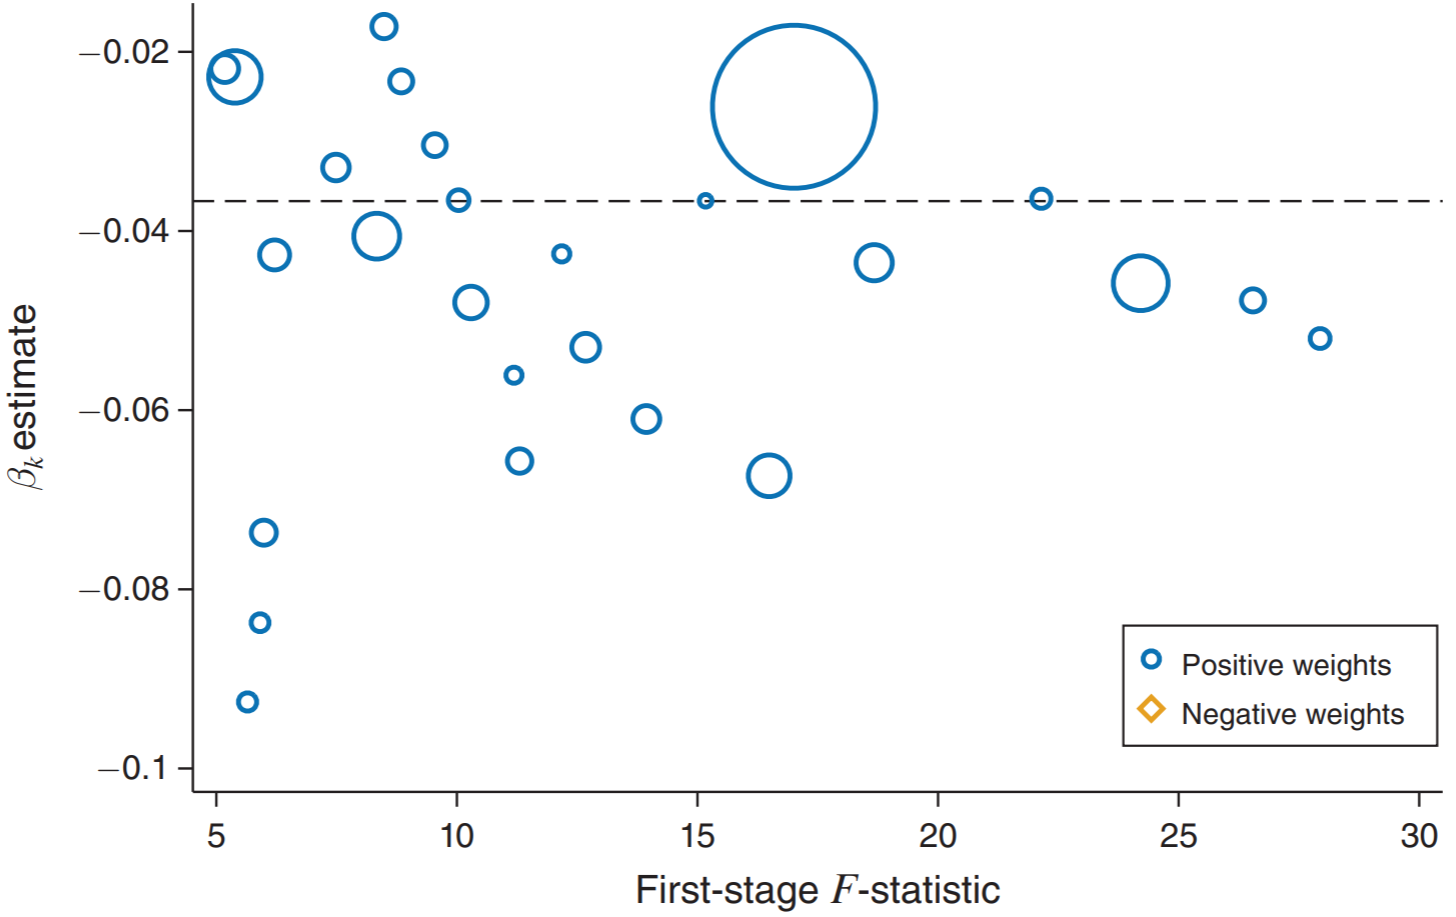
\includegraphics[height=0.8\textheight]{lecture_includes/card_weights.png}
\end{center}
\end{frame}

\begin{frame}{Is Share Exogeneity Plausible?}

Share exogeneity assumption is \textbf{not} that ``shares don't causally respond to the residual'' (they can't: shares are pre-determined)

\begin{itemize}
	\item It's: ``all unobservables are uncorrelated with anything about the local share distribution''
\end{itemize}

\end{frame}

\begin{frame}{Is Share Exogeneity Plausible?}
This sufficient condition is typically violated when there are \emph{any} unobserved shocks $\nu_n$ that affect $\varepsilon_\ell$ via the same or correlated shares
\smallskip
	\begin{itemize}
	%\item Suppose unobserved shocks $\nu_n$ affect $\varepsilon_\ell$ via the same/correlated shares\smallskip\pause
	\item %Share exogeneity is \emph{ex ante} implausible: 
	I.e. if $\varepsilon_\ell=\sum_n s_{\ell n}\nu_n+\tilde{\varepsilon}_\ell$, then $s_{\ell n}$ and $\varepsilon_\ell$ cannot be uncorrelated in large samples---even if $\nu_n$ are uncorelated with $g_n$\smallskip
	\item E.g. in ADH, unobserved technology shocks across industries affect labor markets via lagged emp. shares, along with observed $g_n$\smallskip
	\item Problem arises when shares are ``generic'' -- predicting many things
	\end{itemize}\bigskip
\end{frame}

\begin{frame}{Card and ADH Revisited}

When share exogeneity is \emph{ex ante} plauible, can test its assumptions \emph{ex post} (focusing on high Rotemberg weight $n$):\smallskip

\begin{itemize}
\item Balance/pre-trend tests
\item Overidentification tests (under constant effects)\smallskip
\item Straightforward to implement; no different than any other IV\smallskip
\end{itemize}
\bigskip\pause

GPSS find that balance/overidentification tests broadly pass for Card

 ... but fail badly for ADH, consistent with \emph{ex ante} implausibility
\end{frame}

\section{Choosing an Appropriate Framework}

\begin{frame}{A Taxonomy of SSIV Settings}

\vspace{-4mm}
{\small
\bgPictonBlue{\textbf{Case 1}} the IV is based on a set of shocks which can be thought of as an instrument (i.e. many, plausibly quasi-randomly assigned)
\begin{itemize}
  \item BHJ shows how this identifying variation can be mapped to estimate effects at a different ``level'' (i.e. industries $\rightarrow$ local labor markets)
\end{itemize}

\pause
\bgPictonBlue{\textbf{Case 2}} the researcher does not directly observe many quasi-random shocks, but can estimate them in-sample
\begin{itemize}
  \item Canonical setting of Bartik (1991), where $g_n$ are average industry growth rates (thought to proxy for latent demand shocks)
  \item See also Card (2009), where national immiration rates are estimated
\end{itemize}

\pause
\bgPictonBlue{\textbf{Case 3}} the $g_n$ cannot be naturally viewed as an instrument
\begin{itemize}
  \item Either too few or implausibly exogenous, even given some $q_n$.
  \item Identification may (or may not) instead follow from share exogeneity
\end{itemize}
}



\end{frame}

\begin{frame}{Ex Ante vs. Ex Post Validity}


\vspace{-4mm}
BHJ emphasize that the decision to pursue a ``shocks'' vs. ``shares'' identification strategy must be made \emph{ex ante}
\begin{itemize}
	\item Undesirable to base identifying assumptions on \emph{ex post} tests, though balance/pre-trend tests can be used to falsify assumptions\smallskip
	\item The two identification strategies have different economic content 
\end{itemize}\medskip\pause

They suggest thinking about whether shares are ``tailored'' to the economic question/treatment, or are ``generic''
\begin{itemize}
	\item Generic shares (e.g. ADH): unobserved $\nu_n$ are likely to enter $\varepsilon_\ell$ via the same or similar shares, violating share exogeneity\smallskip
	\item Tailored shares have a diff-in-diff feel; don't even need the shocks, except to possibly improve power or avoid many-IV bias
\end{itemize}

\end{frame}

\end{document}
